% \begin{table}[h!]
% \caption{Exemplo de uma Tabela}
% \label{minhatab}
% \center
% \begin{tabular}{cccc}
%   \hline
% 	Parâmetro & Unidade & Valor da simulação & Valor experimental   \\
% 	\hline
%   Comprimento, $\alpha$ & $m$ &  $8,23$  & $8,54$ \\
%   Altura, $\beta$ & $m$     &  $29,1$ & $28,3$\\
% 	Velocidade, $v$ & $m/s$  &  $60,2$ & $67,3$\\
% 	\hline
% \end{tabular}
% \end{table}

O controle ótimo é uma disciplina fundamental na teoria de controle, com amplas aplicações em diversas áreas da engenharia e ciências aplicadas. Esta teoria lida com o problema de determinar a trajetória de controle que otimiza uma determinada medida de desempenho, sujeita às dinâmicas do sistema e às restrições impostas. A formulação geral do controle ótimo fornece uma base teórica robusta para resolver uma ampla gama de problemas de otimização, desde o controle de veículos autônomos até a gestão de recursos em sistemas complexos.

Neste capítulo, será abordada, inicialmente, a formulação geral do controle ótimo, destacando os princípios e as equações que fundamentam a teoria. Em seguida, explora-se a formulação por colocação direta, uma técnica numérica eficiente para resolver problemas de controle ótimo, com foco especial no método de colocação trapezoidal. Esta abordagem não apenas simplifica a implementação computacional, mas também melhora a precisão e a estabilidade das soluções, tornando-a uma ferramenta valiosa para pesquisadores e profissionais na área de otimização de trajetórias.

\section{Formulação Geral}
\label{sec:formulação-geral}

Segundo \cite{betts_practical_2010}, o Problema de Controle Ótimo pode ser formulado como um conjunto de $N$ fases. Para a fase $i$, o sistema dinâmico pode ser descrito como um conjunto de variáveis dinâmicas

\begin{equation*}
    \mathbf{z} = \left[
        \begin{aligned}
            \mathbf{x}^{(i)}(t) \\
            \mathbf{u}^{(i)}(t)
        \end{aligned}
    \right],
\end{equation*}

\noindent composto por $n_x^{(i)}$ variáveis de estado e por $n_u^{(i)}$ variáveis de controle, respectivamente. Além disso, o sistema pode conter $n_p^{(i)}$ parâmetros $\mathbf{p}^{(i)}$, os quais são independentes de $t$.

Normalmente, as dinâmicas do sistema são definidas por um conjunto de EDOs, chamadas de \textit{equações de estado}:

\begin{equation*}
    \dot{\mathbf{x}}^{(i)} = \mathbf{f}^{(i)} \left[ \mathbf{x}^{(i)}(t), \mathbf{u}^{(i)}(t), \mathbf{p}^{(i)}, t \right].
\end{equation*}

A formulação geral do Problema de Controle Ótimo com $N$ fases utilizada neste trabalho é descrita em \cite{becerra_psopt_2022} e apresentada a seguir.

\subsection*{Problema $\mathcal{P}_1$}
\label{subsec:problema-1}

\noindent Encontrar as trajetórias de controle, $\mathbf{u}^{(i)}(t), \, t \in \left[ t_0^{(i)}, t_f^{(i)} \right]$, trajetórias de estado $\mathbf{x}^{(i)}(t), \, t \in \left[ t_0^{(i)}, t_f^{(i)} \right]$, parâmetros estáticos $\mathbf{p}^{(i)}$ e instantes $t_0^{(i)}, t_f^{(i)}, \, i = 1, \cdots, N$, que minimizem o índice de desempenho $J$, definido pela equação \ref{eq:J}.

\begin{equation}
    \label{eq:J}
    J = \sum_{i=1}^{N} \left[ 
        \varphi^{(i)} \left[ \mathbf{x}^{(i)} \left( t_0^{(i)} \right), \mathbf{x}^{(i)} \left( t_f^{(i)} \right), \mathbf{p}^{(i)}, t_0^{(i)}, t_f^{(i)} \right]
        + \int_{t_0^{(i)}}^{t_f^{(i)}} L^{(i)} \left[ \mathbf{x}^{(i)}(t), \mathbf{u}^{(i)}(t), \mathbf{p}^{(i)}, t \right] \, dt
    \right]
\end{equation}
% In general, an objective function can include two terms: a boundary objective J(·)
% and a path integral along the entire trajectory, with the integrand w(·). A problem
% with both terms is said to be in Bolza form. A problem with only the integral term
% is said to be in Lagrange form, and a problem with only a boundary term is said toDownloaded 06/23/23 to 201.75.182.207 . Redistribution subject to SIAM license or copyright; see https://epubs.siam.org/terms-privacy
% 854
% MATTHEW KELLY
% be in Mayer form [5]. The examples in this paper are all in Lagrange form:
\noindent onde $\varphi(\cdot)$ representa a função objetivo de fronteira e $L(\cdot)$ o integrando da integral de caminho ao longo da trajetória \cite{kelly_introduction_2017}. 

\noindent O problema está sujeito às restrições diferenciais

\begin{equation}
\label{eq:restrições-diferenciais}
    \dot{\mathbf{x}}^{(i)}(t) = \mathbf{f}^{(i)} \left[ \mathbf{x}^{(i)}(t), \mathbf{u}^{(i)}(t), \mathbf{p}^{(i)}, t \right], \, t \in \left[ t_0^{(i)}, t_f^{(i)} \right],
\end{equation}

\noindent às restrições de trajetória

\begin{equation}
\label{eq:restrições-trajetória}
    \mathbf{g}_L^{(i)} \leq \mathbf{g}^{(i)} \left[ \mathbf{x}^{(i)}(t), \mathbf{u}^{(i)}(t), \mathbf{p}^{(i)}, t \right] \leq \mathbf{g}_U^{(i)}, \, t \in \left[ t_0^{(i)}, t_f^{(i)} \right],
\end{equation}

\noindent às restrições de evento

\begin{equation}
\label{eq:restrições-evento}
     \mathbf{e}_L^{(i)} \leq \mathbf{e}^{(i)} \left[ 
     \mathbf{x}^{(i)} \left( t_0^{(i)} \right),
     \mathbf{u}^{(i)} \left( t_0^{(i)} \right),
     \mathbf{x}^{(i)} \left( t_f^{(i)} \right),
     \mathbf{u}^{(i)} \left( t_f^{(i)} \right),
     \mathbf{p}^{(i)}, 
     t_0^{(i)},
     t_f^{(i)} \right] \leq \mathbf{e}_U^{(i)},
\end{equation}

\noindent às restrições de ligação de fase

\begin{equation}
\label{eq:restrições-fase}
\begin{aligned}
    \boldsymbol{\psi}_L \leq \boldsymbol{\psi} [ & \mathbf{x}^{(1)} \left( t_0^{(1)} \right), \mathbf{u}^{(1)} \left( t_0^{(1)} \right), \\
        & \mathbf{x}^{(1)} \left( t_f^{(1)} \right), \mathbf{u}^{(1)} \left( t_f^{(1)} \right), \mathbf{p}^{(1)}, t_0^{(1)}, t_f^{(1)}, \\
        & \mathbf{x}^{(2)} \left( t_0^{(2)} \right), \mathbf{u}^{(2)} \left( t_0^{(2)} \right), \\
        & \mathbf{x}^{(2)} \left( t_f^{(2)} \right), \mathbf{u}^{(2)} \left( t_f^{(2)} \right), \mathbf{p}^{(2)}, t_0^{(2)}, t_f^{(2)}, \\
        & \vdots \\
        & \mathbf{x}^{(N)} \left( t_0^{(N)} \right), \mathbf{u}^{(N)} \left( t_0^{(N)} \right), \\
        & \mathbf{x}^{(N)} \left( t_f^{(N)} \right), \mathbf{u}^{(N)} \left( t_f^{(N)} \right), \mathbf{p}^{(N)}, t_0^{(N)}, t_f^{(N)} ] \leq \boldsymbol{\psi}_U ,
\end{aligned}
\end{equation}

\noindent às restrições de limite

\begin{gather}
    \mathbf{u}_L^{(i)} \leq \mathbf{u}^{(i)}(t) \leq \mathbf{u}_U^{(i)}, \, t \in \left[ t_0^{(i)}, t_f^{(i)} \right], \nonumber \\
    \mathbf{x}_L^{(i)} \leq \mathbf{x}^{(i)}(t) \leq \mathbf{x}_U^{(i)}, \, t \in \left[ t_0^{(i)}, t_f^{(i)} \right], \nonumber \\
    \mathbf{p}_L^{(i)} \leq \mathbf{p}^{(i)} \leq \mathbf{p}_U^{(i)}, \\
    t_{0_L}^{(i)} \leq t_0^{(i)} \leq t_{0_U}^{(i)}, \nonumber \\
    t_{f_L}^{(i)} \leq t_f^{(i)} \leq t_{f_U}^{(i)}, \nonumber
\end{gather}

\noindent e às seguintes restrições

\begin{equation}
\begin{aligned}
    t_f^{(i)} &- t_0^{(i)} \geq 0, \, i = 1, \cdots, N \\
    \mathbf{u}^{(i)} &: \left[ t_0^{(i)}, t_f^{(i)} \right] \rightarrow \mathbb{R}^{n_u^{(i)}} \\
    \mathbf{x}^{(i)} &: \left[ t_0^{(i)}, t_f^{(i)} \right] \rightarrow \mathbb{R}^{n_x^{(i)}} \\
    \mathbf{p}^{(i)} &\in \mathbb{R}^{n_p^{(i)}} \\
    \varphi^{(i)} &: \mathbb{R}^{n_x^{(i)}} \times \mathbb{R}^{n_x^{(i)}} \times \mathbb{R}^{n_p^{(i)}} \times \mathbb{R} \times \mathbb{R} \rightarrow \mathbb{R} \\
    L^{(i)} &: \mathbb{R}^{n_x^{(i)}} \times \mathbb{R}^{n_u^{(i)}} \times \mathbb{R}^{n_p^{(i)}} \times \left[ t_0^{(i)}, t_f^{(i)} \right] \rightarrow \mathbb{R} \\
    \mathbf{f}^{(i)} &: \mathbb{R}^{n_x^{(i)}} \times \mathbb{R}^{n_u^{(i)}} \times \mathbb{R}^{n_p^{(i)}} \times \left[ t_0^{(i)}, t_f^{(i)} \right] \rightarrow \mathbb{R}^{n_x^{(i)}} \\
    \mathbf{g}^{(i)} &: \mathbb{R}^{n_x^{(i)}} \times \mathbb{R}^{n_u^{(i)}} \times \mathbb{R}^{n_p^{(i)}} \times \left[ t_0^{(i)}, t_f^{(i)} \right] \rightarrow \mathbb{R}^{n_g^{(i)}} \\
    \mathbf{e}^{(i)} &: \mathbb{R}^{n_x^{(i)}} \times \mathbb{R}^{n_u^{(i)}} \times \mathbb{R}^{n_x^{(i)}} \times \mathbb{R}^{n_u^{(i)}} \times \mathbb{R}^{n_p^{(i)}} \times \mathbb{R} \times \mathbb{R} \rightarrow \mathbb{R}^{n_e^{(i)}} \\
    \boldsymbol{\psi} &: U_{\Psi} \rightarrow \mathbb{R}^{n_{\Psi}}
\end{aligned}
\end{equation}

\noindent onde $U_{\Psi}$ é o domínio da função $\boldsymbol{\psi}$.

\section{Formulação por Colocação Direta}
\label{sec:formulação-coloc-direta}

Os métodos diretos discretizam o PCO, de forma a converte-lo em um problema de PNL. Tal processo é conhecido como transcrição. Para isso, as funções contínuas do problema serão aproximadas por \textit{splines}, as quais são funções compostas por vários segmentos polinomiais \cite{kelly_introduction_2017}.

Antes de apresentar a discretização das funções usando a colocação trapezoidal, faz-se necessário apresentar o problema de PNL. Tais problemas contêm um ou mais termos não-lineares, seja na sua função objetivo ou nas suas restrições. A típica formulação de um problema de PNL é apresentado na equação \ref{eq:PNL}.

\begin{equation}
\label{eq:PNL}
    \begin{aligned}
        \min_\mathbf{z} J(\mathbf{z}) \qquad &\text{sujeito a} \\
        & \mathbf{f}(\mathbf{z}) = \mathbf{0}, \\
        & \mathbf{g}(\mathbf{z}) \leq \mathbf{0}, \\
        & \mathbf{z}_L \leq \mathbf{z} \leq \mathbf{z}_U
    \end{aligned}
\end{equation}

% Visando um formato que se encaixe na descrição de um problema de PNL, como apresentado, iniciamos a discretização das funções do PCO.
Por simplicidade e clareza, dispensaremos a notação $(i)$, indicativa da fase, na sequência deste documento. Iniciando a discretização das funções do PCO, seguindo o exposto em \cite{betts_practical_2010}, a duração da fase é dividida em $n_s$ segmentos

\begin{equation}
    \label{eq:tempo-disc}
    t_0 = t_1 < t_2 < \cdots < t_M = t_f,
\end{equation}

\noindent onde cada ponto é chamado de \textit{nó}. O número de nós é dado por $M \equiv n_s + 1$. Quanto às variáveis do problema, a notação utilizada será $\mathbf{x}_k \equiv \mathbf{x}(t_k)$ para as variáveis de estado e $\mathbf{u}_k \equiv \mathbf{u}(t_k)$ para as variáveis de controle. Além disso, denota-se $\mathbf{f}_k \equiv \mathbf{f} \left[ \mathbf{x}(t_k), \mathbf{u}(t_k), \mathbf{p}, t_k \right]$.
% $\overline{\mathbf{u}}_k \equiv \mathbf{u}(\overline{t})$ com $\overline{t} = \frac{1}{2} \left( t_k + t_{k-1} \right)$ como o valor da variável de controle no ponto-médio de um intervalo.

Dessa forma, visando a transcrição para um problema de PNL, as equações diferenciais do PCO são substituídas por um conjunto de restrições. Assim, as restrições do PCO - equações \ref{eq:restrições-diferenciais} a \ref{eq:restrições-evento} - serão substituídas pelas restrições do problema de PNL:

\begin{equation}
    \mathbf{c}_L \leq \mathbf{c}(\mathbf{x}) \leq \mathbf{c}_U,
\end{equation}

\noindent onde

\begin{equation}
\begin{aligned}
    \mathbf{c}(\mathbf{x}) =& \left[ \boldsymbol{\zeta}_1, \boldsymbol{\zeta}_2, \cdots, \boldsymbol{\zeta}_{M-1}, \mathbf{g}_1, \mathbf{g}_2, \cdots, \mathbf{g}_{M}, \mathbf{e}_0, \mathbf{e}_f, \boldsymbol{\psi}_0, \boldsymbol{\psi}_f \right]^\intercal \\
    \mathbf{c}_L =& \left[ \mathbf{0}, \cdots, \mathbf{0}, \mathbf{g}_L, \cdots, \mathbf{g}_L, \mathbf{e}_L, \mathbf{e}_L, \boldsymbol{\psi}_L, \boldsymbol{\psi}_L \right]^\intercal \\
    \mathbf{c}_U =& \left[ \mathbf{0}, \cdots, \mathbf{0}, \mathbf{g}_U, \cdots, \mathbf{g}_U, \mathbf{e}_U, \mathbf{e}_U, \boldsymbol{\psi}_U, \boldsymbol{\psi}_U \right]^\intercal
\end{aligned}
\end{equation}

As primeiras $n_x n_s$ restrições exigem que os vetores $\boldsymbol{\zeta}$ sejam zero, satisfazendo aproximadamente as equações diferenciais do PCO - dadas pela equação \ref{eq:restrições-diferenciais}.


\subsection{Colocação Trapezoidal}

Focando no método trapezoidal, a variável de controle é discretizada usando uma \textit{spline} linear 

\begin{equation}
    \mathbf{u}(t) \approx \mathbf{u}_k + \dfrac{\tau}{h_k} (\mathbf{u}_{k+1} - \mathbf{u}_k),
\end{equation}

\noindent onde $\tau \equiv t - t_k$ e $h_k \equiv t_{k+1} - t_k$, e a variável de estado é discretizada usando uma \textit{spline} quadrática

\begin{equation}
    \mathbf{f}(t) = \dot{\mathbf{x}}(t) \approx \mathbf{f}_k + \dfrac{\tau}{h_k} (\mathbf{f}_{k+1} - \mathbf{f}_k),
\end{equation}

\noindent que, ao ser integrada, resulta em

\begin{equation}
    \mathbf{x}(t) \approx \mathbf{x}_k + \mathbf{f}_k \tau + \dfrac{\tau^2}{2h_k} (\mathbf{f}_{k+1} - \mathbf{f}_k).
\end{equation}

\begin{figure}[H]
    \centering
    \begin{subfigure}{0.48\linewidth}
        \centering
        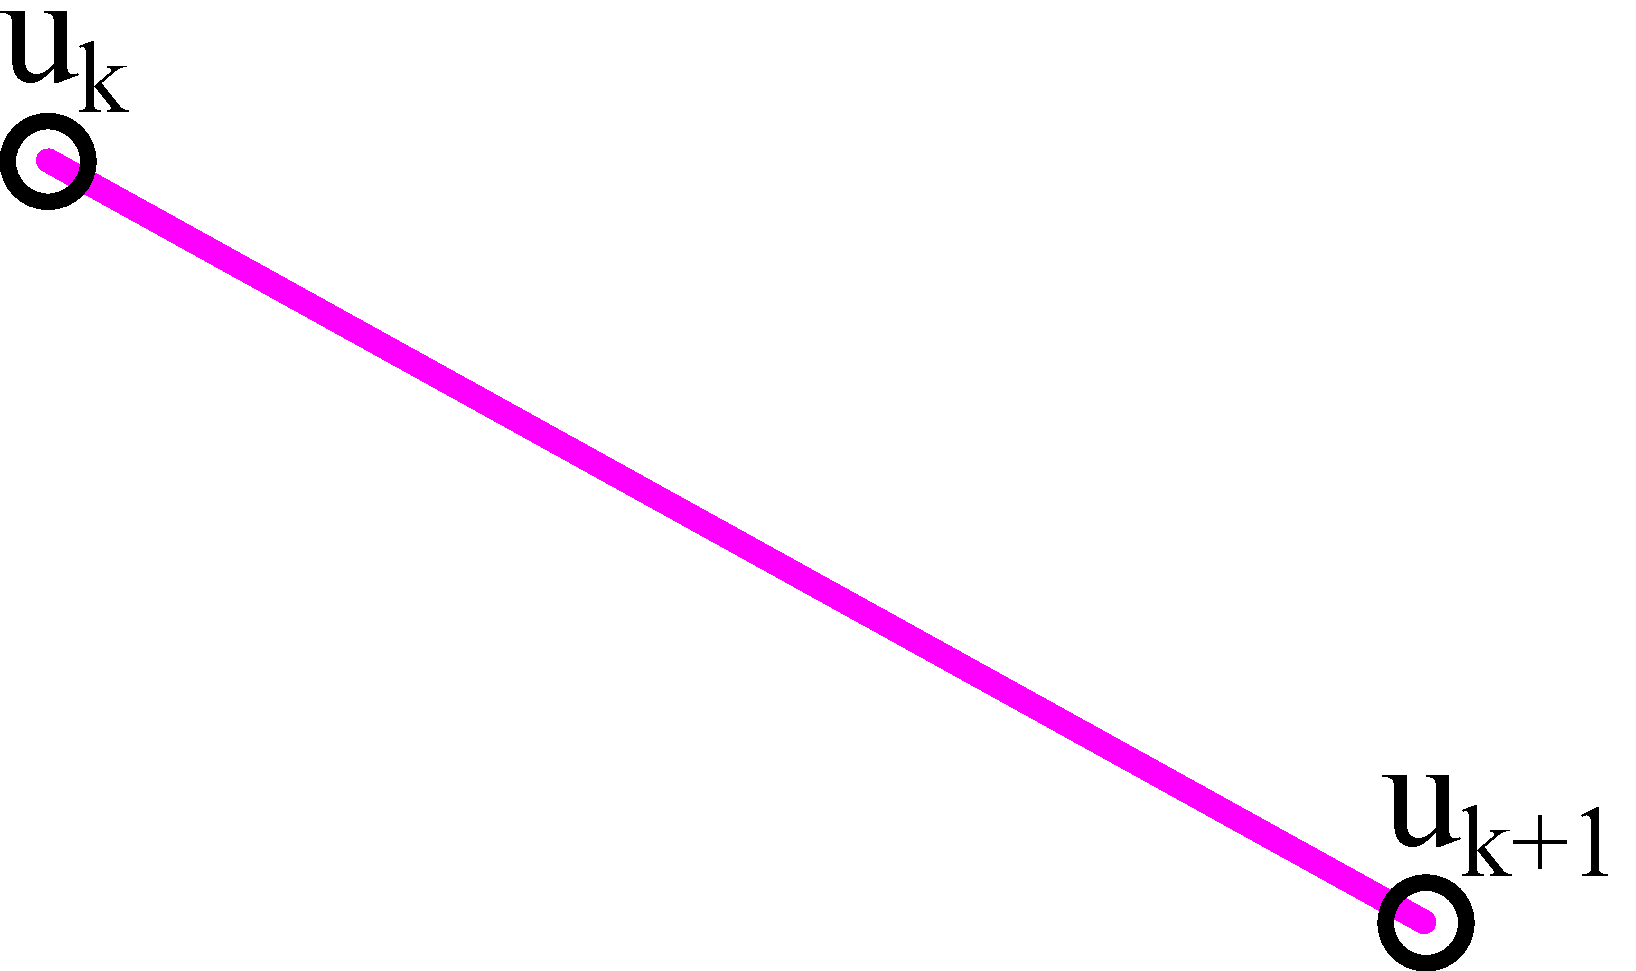
\includegraphics[width=0.7\textwidth]{Cap2/linear-spline.pdf}
        \caption{\textit{Spline} linear de controle}
    \end{subfigure}
    \hfill
    \begin{subfigure}{0.48\linewidth}
        \centering
        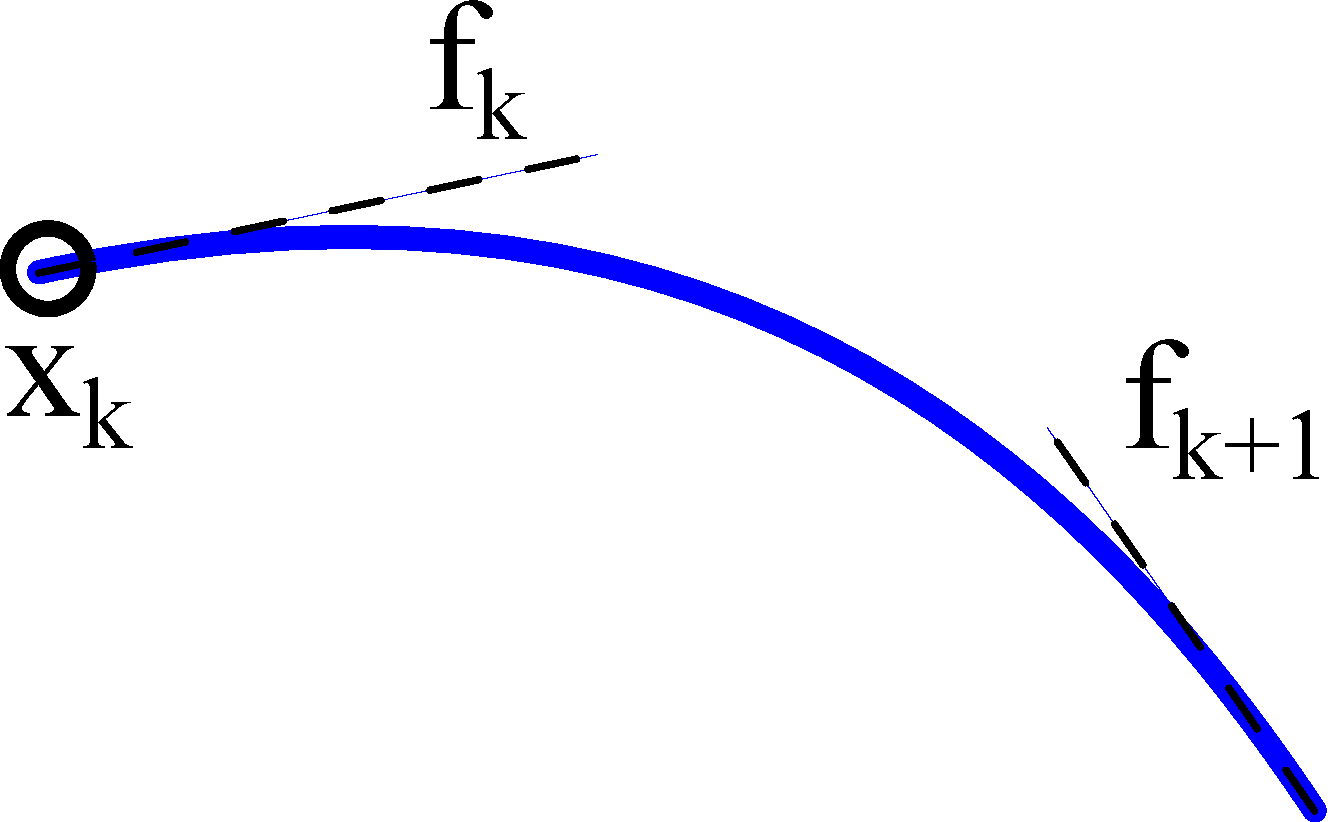
\includegraphics[width=0.57\textwidth]{Cap2/quadratic-spline.pdf}
        \caption{\textit{Spline} quadrática de estado}
    \end{subfigure}
    % \includegraphics[width=0.8\textwidth]{Cap2/}
    \caption{Representações das \textit{splines} de controle e de estado}
    \label{fig:splines}
\end{figure}

Desse modo, as variáveis são definidas como

\begin{equation}
    \mathbf{z}^\intercal = \left( \mathbf{x}_1, \mathbf{u}_1, \cdots, \mathbf{x}_M, \mathbf{u}_M \right)
\end{equation}

\noindent e as restrições

\begin{equation}
    \boldsymbol{\zeta}_k = \mathbf{x}_{k+1} - \mathbf{x}_k - \dfrac{h_k}{2} \left( \mathbf{f}_{k+1} + \mathbf{f}_k \right)
\end{equation}

Assim, pode-se reescrever o índice de desempenho - equação \ref{eq:J} - como

\begin{equation}
    J = \varphi \left[ \mathbf{x} \left( t_0 \right), \mathbf{x} \left( t_f \right), \mathbf{p}, t_0, t_f \right]
    + \sum_{k=0}^{M-1} \dfrac{1}{2} h_k \left( L_{k+1} + L_k \right)
\end{equation}


